% !TEX root = ./Basilisk-pixelLineConverter-20190524.tex


\begin{figure}[H]
	\centerline{
		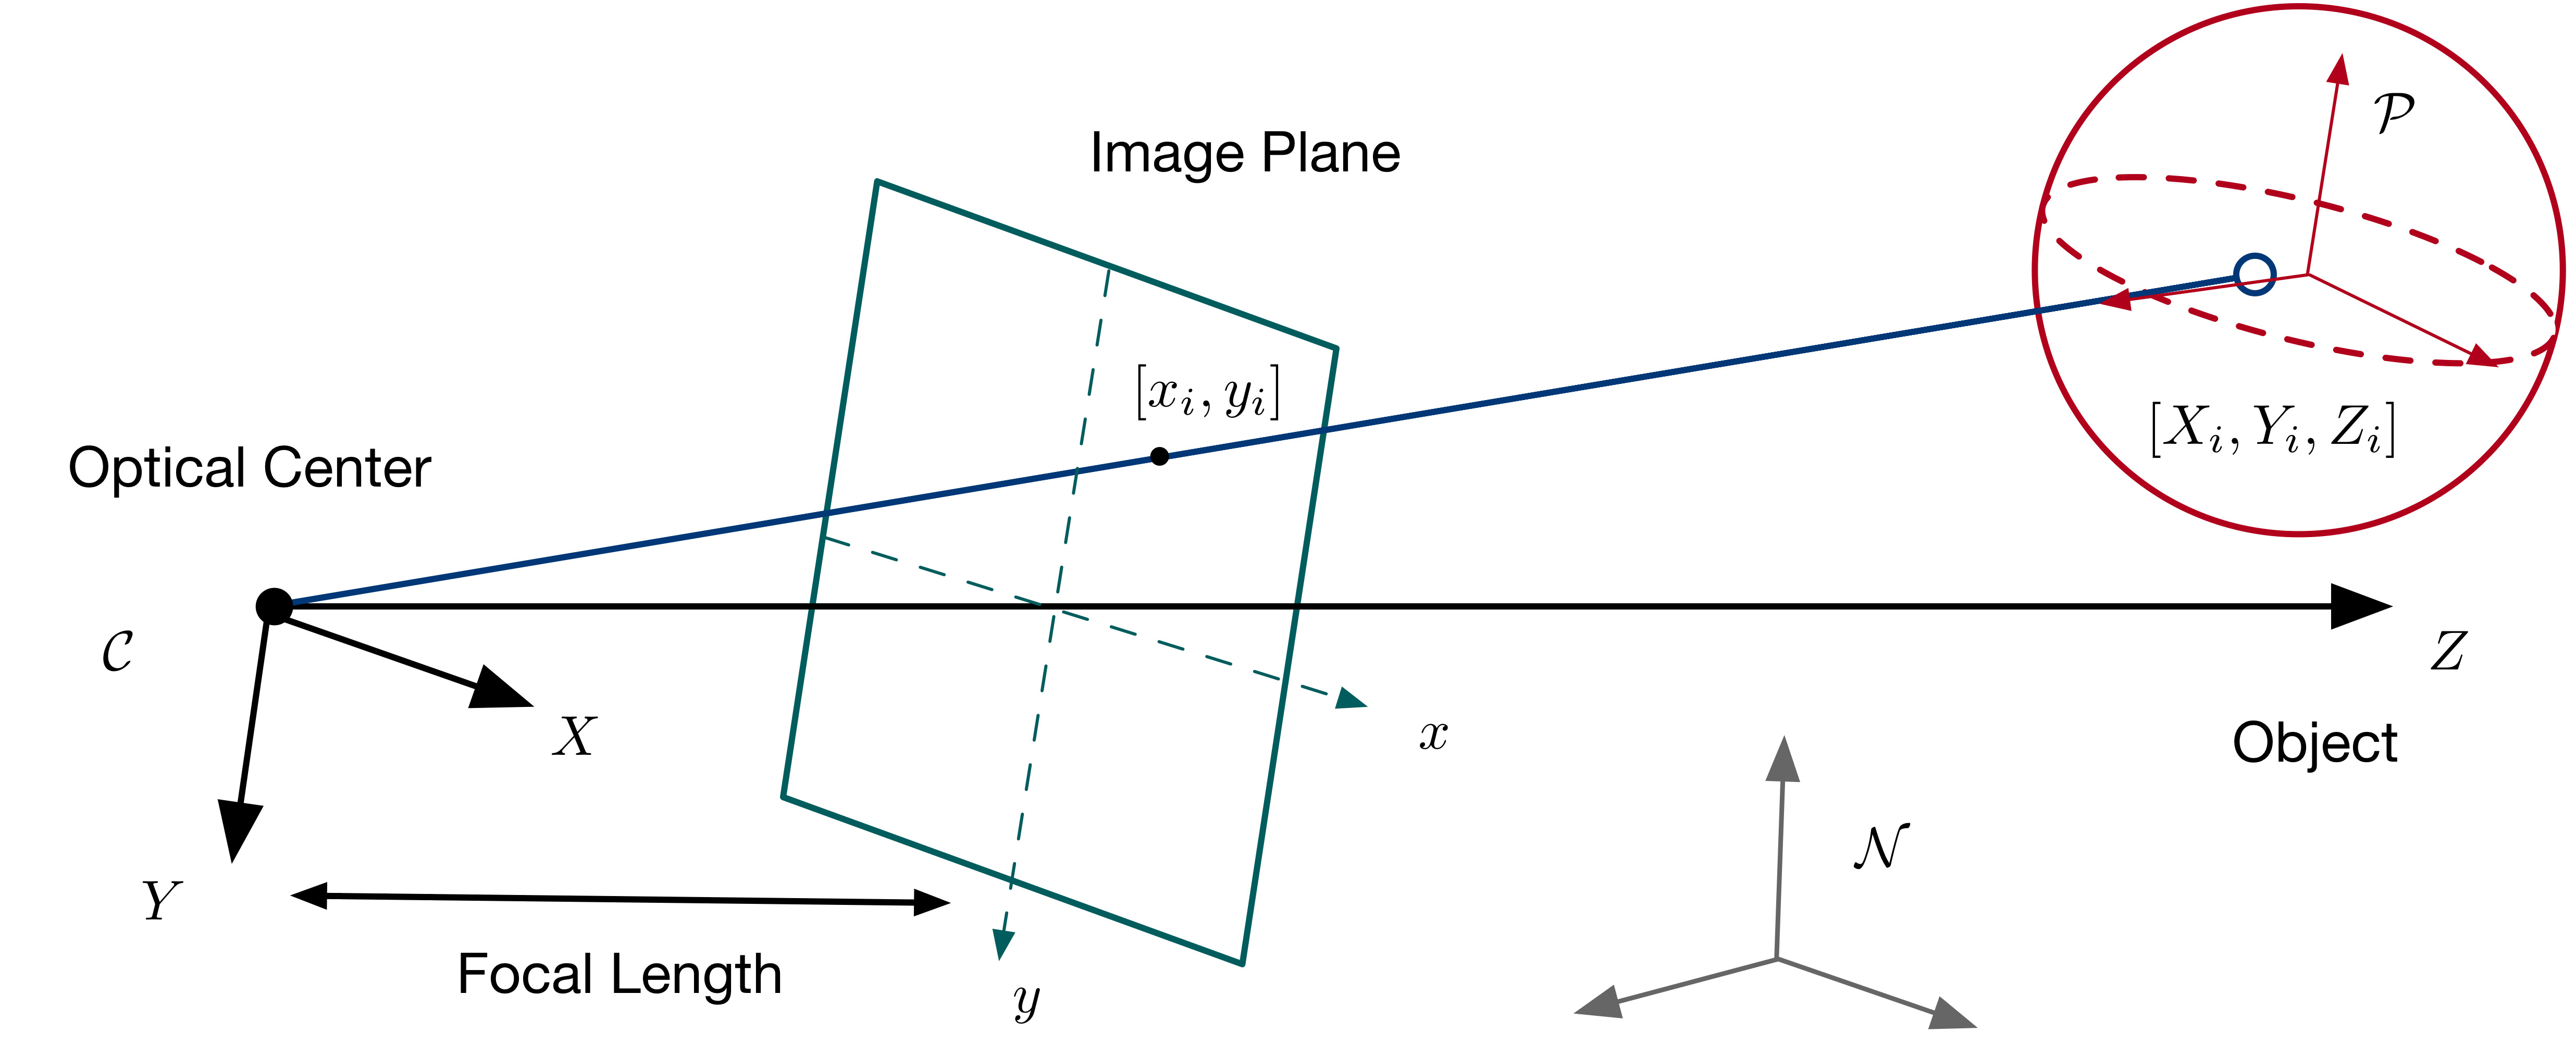
\includegraphics{Figures/CameraGeometry}
	}
	\caption{Camera Model}
	\label{fig:camera}
\end{figure}

\section{Model Description}

\subsection{Input and Output}

This converter module processes the output of a circle finding method to extract spacecraft inertial position. It does this by reading spacecraft attitude (coming from star tracker or other means), camera parameters, and the circle properties. 

Messages read:

\begin{itemize}
\item CameraConfigInMsg: containing focal length, resolution, and sensor size. These values are needed for the following computations. Notably the camera frame relative to the body frame is used.
\item CirclesInMsg: Circle radius, center pixel and line, and uncertainty around these values in pixels. 
\item NavAttInMsg: Used for the spacecraft attitude. This allows to move from the body frame to the inertial frame.
\end{itemize}

Message written:
\begin{itemize}
\item OpNavMsgPayload: Message containing $\leftexp{N}{\bm r}$ and it's covariance.
\end{itemize}

\subsection{Position computation}

A geometrical method can be used to extract pose information from center and apparent diameter information. The norm of the position vector is given by the apparent size, it's direction is given by the pixel and line data. Using $\leftexp{C}{\bm r_c} = \leftexp{C}{\begin{bmatrix} r_1 & r_2 & r_3 \end{bmatrix}}^T$ as the relative vector of the camera with respect to the celestial center, $A$ as the apparent diameter of the celestial body, $D$ as the actual diameter:

\begin{align}\label{eq:cad}
|\bm r_c| = \frac{1}{2}\frac{D}{\sin\left(\frac{1}{2} A\right)} \hspace{2cm} \frac{1}{r_3}\begin{bmatrix} r_1 \\ r_2 \end{bmatrix}= \frac{1}{r_3}\tilde{\bm r} = \frac{1}{f}\begin{bmatrix} x \\ y \end{bmatrix}
\end{align}

These equations have been used in multiple instances~\cite{Battin, Owen_OpNav}. The third component of $\bm r_c$ provides the range measurement to the body which can be extracted using the apparent diameter measurements. Hence the definition of $\tilde{\bm r}$ which only contains the first two components of $\bm r_c$. The vector components of $\bm r_{c}$ can be expressed relative to the inertial frame assuming inertial attitude knowledge from other instruments. Using the position of the camera on the spacecraft this provides the measurement value for an orbit determination filter using a circle-finding algorithm.  

\subsection{Uncertainty computation}

In the case of the geometric formula, the partials allow to quantify error due to the camera specifications. Indeed, if $X, Y$ the pixel sizes (in their respective directions), $x,y$ are the position on the camera, and $x_i, y_i, \rho_i$ the pixel values for the CAD measurements:
\begin{equation}\label{eq:pl2vector}
\tilde{\bm r} =\frac{r_3}{f} \begin{bmatrix} x \\ y \end{bmatrix} =\frac{r_3}{f} \begin{bmatrix} x_i X \\ y_i Y \end{bmatrix} 
\end{equation}
\begin{equation}\label{eq:mag2rho}
|\bm r_c| = \frac{1}{2}\frac{D}{\sin\left(\frac{1}{2} A\right)} = \frac{1}{2}\frac{D}{\sin\left( \arctan \left( \frac{\rho}{f}\right)\right)} = \frac{1}{2}\frac{D}{\sin\left(\arctan \left( \frac{\rho_i X}{f}\right)\right)} 
\end{equation}
Eq.~\eqref{eq:pl2vector} provides a simple partial with respect to the measurement $\bm c_i = \begin{bmatrix} x_i & y_i\end{bmatrix}^T$
\begin{equation}
\frac{\partial \tilde{\bm r}}{\partial \bm c_i } = r_3\begin{bmatrix} \frac{X}{f} & 0 \\ 0 & \frac{Y}{f} \end{bmatrix} \hspace{0.5cm}\Rightarrow \hspace{0.5cm}\mathbb{E}\left[ \delta \tilde{\bm r} \delta  \tilde{\bm r}^T \right] =  r_3^2\begin{bmatrix} \frac{X}{f} & 0 \\ 0 & \frac{Y}{f} \end{bmatrix} \left[ \delta \bm c_i \delta \bm c_i ^T \right]  \begin{bmatrix} \frac{X}{f} & 0 \\ 0 & \frac{Y}{f} \end{bmatrix} 
\end{equation}
The partial for Eq.~\eqref{eq:mag2rho} is:
\begin{align}
\frac{\partial |\bm r_c|}{\partial \rho_i } = \frac{Dd_x}{2} \sqrt{f^2+ \rho^2 d_x^2}\left(\frac{1}{f^2+ \rho^2d_x^2}-\frac{1}{\rho^2 d_x^2} \right)
\end{align}